\documentclass{article}

\usepackage[spanish]{babel}
\selectlanguage{spanish}
\usepackage[utf8]{inputenc}
\usepackage[pdftex]{graphicx}

% Utilizado para recuadrar expresiones
\usepackage{amsmath}
% Recuadros con mayor separación
\setlength{\fboxsep}{6pt}

\def \anio {a\tilde{n}o}

\title{Trabajo Práctico 2\\Administración de Stocks}
\author{}
\date{\today}

%%% Agregar integrantes del grupo %%%

\begin{document}
\maketitle

%%%% Poner el enunciado aca.. y un indice %%%%
\paragraph{Ejercicio 4}
    Los datos proporcionados son la demanda anual $ D = 20000 u $, el costo de setup $ K = \$6000 $, el costo de almacenamiento $ C_1 = \$20\ u^{-1}\ \anio^{-1} $ y la tasa de producción $ p = 5000u\ mes^{-1} = 60000u\ \anio^{-1}$.

    \paragraph{4.a}
    El modelo elegido para este problema es el Modelo de Reposición no Instantánea. Se asumen las siguientes hipótesis:
        \begin{itemize}
            \item Se administra un solo producto.
            \item La demanda es conocida y constante.
            \item No hay descuentos por cantidad.
            \item No hay inflación.
            \item La producción se efectúa a tasa conocida y constante.
            \item No se admite agotamiento.
            \item No hay stock de protección.
            \item Costo de setup independiente del tamaño del lote.
            \item Costo unitario de almacenimiento independiente del stock.
            \item Se supone continuidad permanente de operación.
        \end{itemize}

    \paragraph{4.b.} 
        $$ q_o = \sqrt{ \frac{2KD}{TC_1 \left( 1 - \frac{d}{p} \right)} } $$
        $$ q_o = \sqrt{ \frac{2 \cdot \$ 6000 \cdot 20000u\ \anio^{-1}}{\$20 u^{-1}\ \anio^{-1} \left( 1 - \frac{20000u\ \anio^{-1}}{60000u\ \anio^{-1}} \right)} } $$
        $$ q_o = \sqrt{ \frac{2 \cdot 6 \cdot 10^6\ u^2}{1 - \frac{2}{6}} } = \sqrt{ \frac{2 \cdot 6 \cdot 10^6}{\frac{2}{3}} }\ u = \sqrt{ 3 \cdot 6 \cdot 10^6 }\ u $$
        $$ \boxed{ q_o = 3 \cdot 10^3 \sqrt {2}\ u \simeq 4242.64\ u } $$

    \paragraph{4.c.}
        Como se indica en el item h, se consideran 20 días por mes.
        
        $$ \frac{T}{t_i} = \frac{D}{q} \Rightarrow t_i = \frac{Tq}{D} $$
        $$ t_i = \frac{3 \cdot 10^3 \sqrt{2}\ u}{20000u\ \anio^{-1}} = \frac{3 \sqrt{2}\ \anio}{20} \frac{240 dias}{\anio} $$
        $$ \boxed{ t_i = 36 \sqrt{2} dias \simeq 50.91\ dias } $$
    
    \paragraph{4.d.}
        $$ CTE_o = bD + \sqrt{ 2KDTC_1 \left( 1 - \frac{d}{p} \right) } = \sqrt{ 2KDTC_1 \left( 1 - \frac{d}{p} \right) } $$
        $$ CTE_o = \sqrt{ 2\ \$6000 \cdot 20000u\ \anio^{-1}\ \$20u^{-1}\anio^{-1} \cdot \frac{2}{3} } = \$2 \sqrt{ \frac{24 \cdot 10^8}{3} } = \$2 \cdot 10^4 \sqrt{8} $$
        $$ \boxed{ CTE_o = \$4 \cdot 10^4 \sqrt{2} \simeq \$ 56568.54 } $$

    \paragraph{4.e.}
        $$ n = \frac{D}{q} = \frac{20000u}{3 \cdot 10^3 \sqrt{2}\ u} $$
        $$ \boxed{ n = \frac{20}{3 \sqrt{2}} \simeq 4.714 } $$
    
    \paragraph{4.f.}
        $$ S_o = q_o \left( 1 - \frac{d}{p} \right) = 3 \cdot 10^3 \sqrt {2}\ u \cdot \frac{2}{3} $$
        $$ \boxed{ S_o = 2 \cdot 10^3 \sqrt {2}\ u \simeq 2828.43 u } $$
    
    \paragraph{4.g.}
        Lo que se pide es el tiempo de producción de una orden $ t_{ip} $ y el tiempo de demanda únicamente de una orden $ t_{id} $. Como se indica en el item h, se consideran 20 días por mes.
        
        $$ t_{ip} = \frac{q}{p} = \frac{3 \cdot 10^3 \sqrt {2}\ u}{60000u\ \anio^{-1}} = \frac{3 \sqrt {2}\ \anio}{60} = \frac{\sqrt{2}\ \anio}{20} \cdot \frac{240dias}{\anio}$$
        $$ \boxed{ t_{ip} = 12\sqrt{2}\ dias \simeq 16.97\ dias } $$
        
        $$ t_{id} = \frac{S}{d} = \frac{2 \cdot 10^3 \sqrt {2}\ u}{20000u\ \anio^{-1}} = \frac{\sqrt{2}\ \anio}{10} \cdot \frac{240\ dias}{\anio} $$
        $$ \boxed{ t_{id} = 24\sqrt{2}\ dias \simeq 33.94\ dias } $$
    
    \paragraph{4.h.}
        $$ LT = 2\ dias \leq 33.94\ dias = t_{id} \Rightarrow S_R = LT \cdot d $$
        $$ S_R = \frac{2\ dias \cdot 20000u}{\anio} \cdot \frac{\anio}{240\ dias} = \frac{2 \cdot 20000u}{240} = \frac{2000u}{12} $$
        $$ \boxed{S_R = 166.\overline{6} u} $$

\pagebreak

\paragraph{Ejercicio 7}
Se trata de un caso de modelo básico (ver ejercicio 1) de un solo ítem, demanda constante, agotamiento no admitido, donde el costo de almacenamiento $C_{1}$ crece mediante la siguiente ley:
\begin{center}
  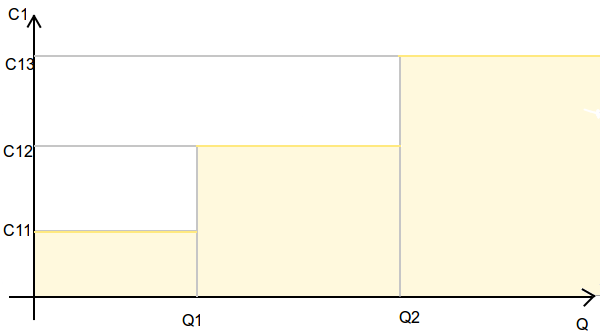
\includegraphics[scale=0.4,keepaspectratio=true]{img/7/7_QvsC1.png} 
\end{center}
Se sabe que para este modelo:
  \begin{equation}\label{7_CTE}CTE_i = bD + \frac{1}{2}qC_{1i}T + K\frac{D}{q} \end{equation}
  $$ q_{oi} = \sqrt{ \frac{2KD}{TC_{1i}}} $$
  $$ CTE_{oi} = bD + \sqrt{ 2KDC_{1i}T }$$

Con lo cual, se deduce la siguiente relacion entre variables:
 $$ C_{11} < C_{12} < C_{13} $$
 $$ q_{o1} > q_{o2} > q_{o3}$$
 $$ CTE_{o1} < CTE_{o2} < CTE_{o3} $$
 
El procedimiento a seguir para la búsqueda del costo total esperado mínimo es el siguiente: 
\begin{enumerate}
 \item si $q_{o1} < Q_1 \Rightarrow CTE_o = CTE_{o1}$ \\
      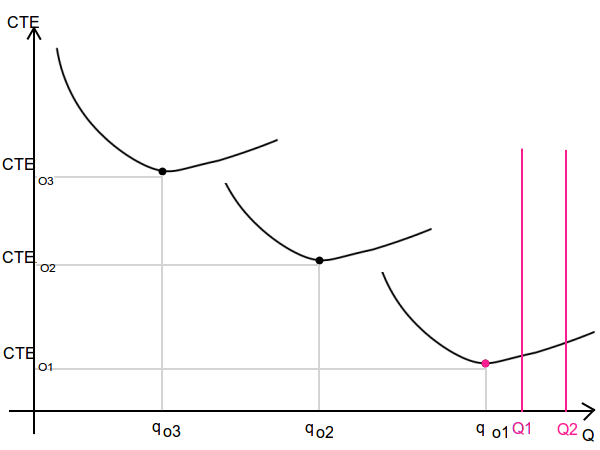
\includegraphics[scale=0.5,keepaspectratio=true]{img/7/7_QvsCTE_1.png} 
 \item sino, si $ q_{o2} < Q_1 \Rightarrow CTE_o = min( CTE(Q_1, C_{12}), CTE(Q_1, C_{11})$ \\
       Se entiende por $CTE(Q_i, C_{1i})$ el costo total esperado \eqref{7_CTE} evaluado en $Q_i$ y $C_{1i}$ \\
      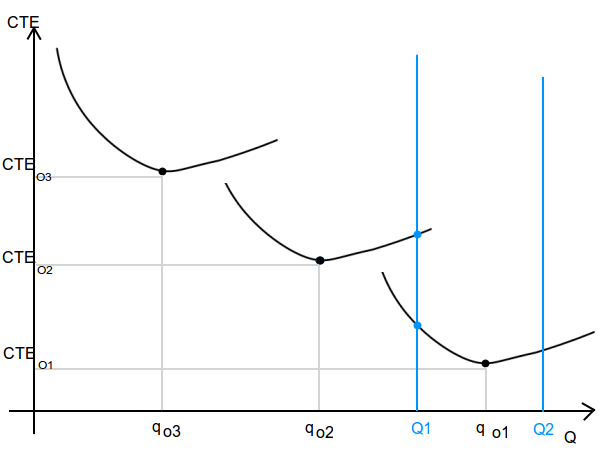
\includegraphics[scale=0.5,keepaspectratio=true]{img/7/7_QvsCTE_2.png} 
 \item sino, si $ Q_1 < q_{o2} < Q_2 \Rightarrow CTE_o = min( CTE_{o2}, CTE(Q_1, C_{11})) $ \\
      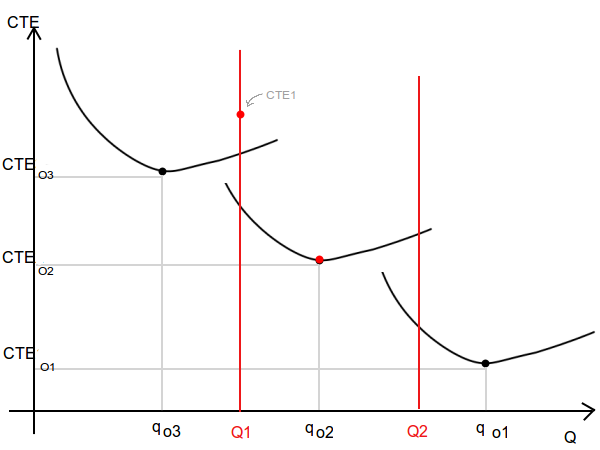
\includegraphics[scale=0.5,keepaspectratio=true]{img/7/7_QvsCTE_3.png} 
 \item sino, si $q_{o3} < Q_1 \Rightarrow CTE_o = min( CTE(Q_2, C_{12}), CTE(Q_2, C_{13}), CTE(Q_1, C_{11})) $ \\
      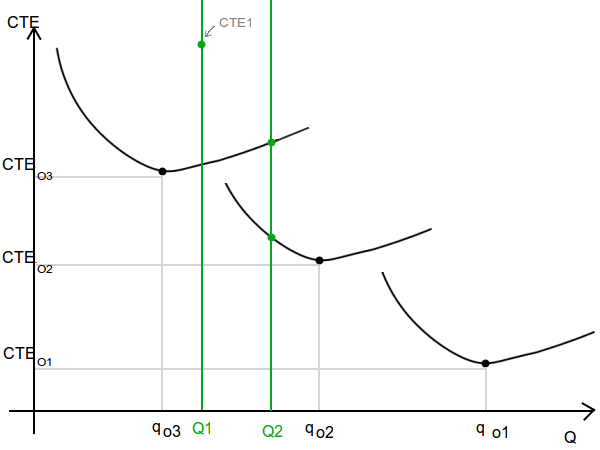
\includegraphics[scale=0.5,keepaspectratio=true]{img/7/7_QvsCTE_4.png} 
 \item sino, $q_{o3} > Q_2 \Rightarrow CTE_o = min(CTE_{o3},CTE(Q_2, C_{12}), CTE(Q_1, C_{11}) ) $ \\
      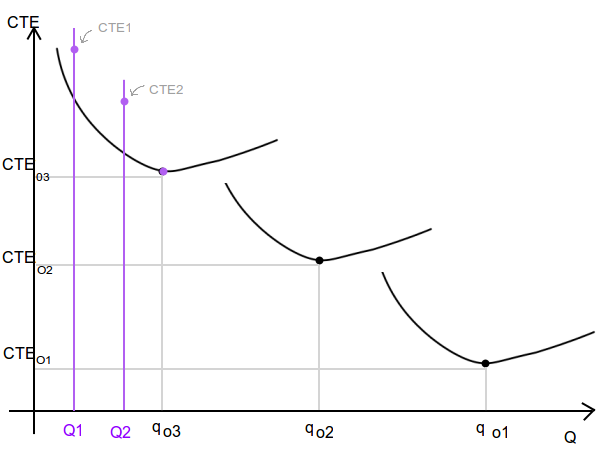
\includegraphics[scale=0.5,keepaspectratio=true]{img/7/7_QvsCTE_5.png} 
 \end{enumerate}

Para cada uno de estos casos, el costo total esperado en función de q está dado por la curva naranja, donde cada $CTE_i$ es válido dentro de su rango. 
\begin{enumerate}
 \item 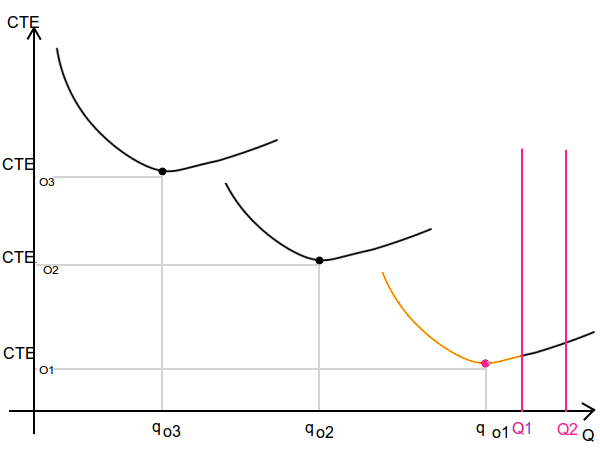
\includegraphics[scale=0.4,keepaspectratio=true]{img/7/7_QvsCTE_1B.png} 
 \item 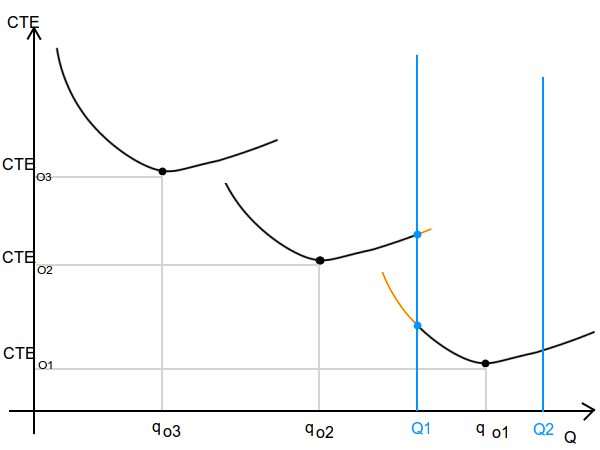
\includegraphics[scale=0.4,keepaspectratio=true]{img/7/7_QvsCTE_2B.png} 
 \item 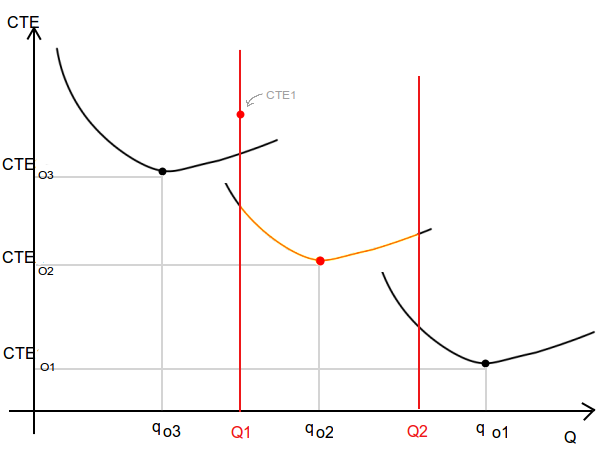
\includegraphics[scale=0.4,keepaspectratio=true]{img/7/7_QvsCTE_3B.png} 
 \item 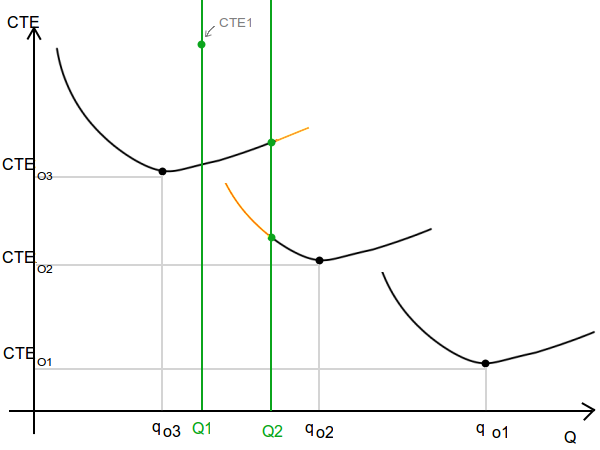
\includegraphics[scale=0.4,keepaspectratio=true]{img/7/7_QvsCTE_4B.png} 
 \item 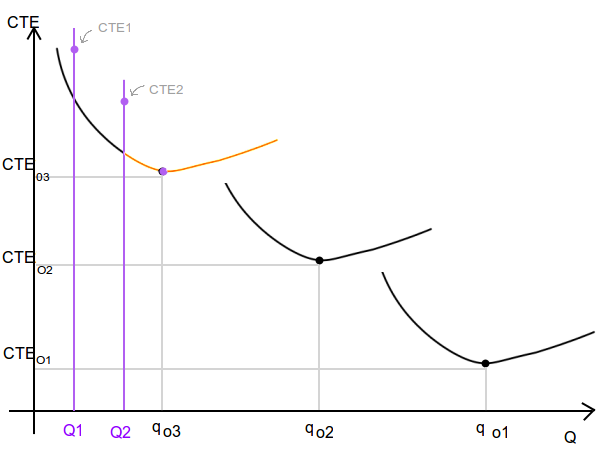
\includegraphics[scale=0.4,keepaspectratio=true]{img/7/7_QvsCTE_5B.png} 
\end{enumerate}


\paragraph{Ejercicio 8}
Se trata de un caso de modelo básico (ver ejercicio 1) de un solo ítem, demanda constante, agotamiento no admitido y con K creciente mediante la siguiente ley: 
\begin{center}
  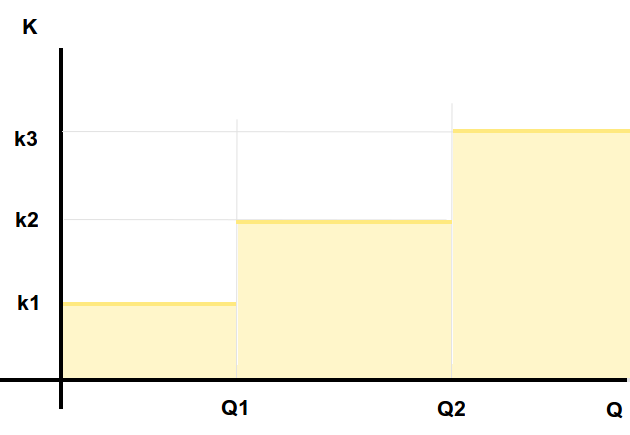
\includegraphics[scale=0.4,keepaspectratio=true]{img/8/8_QvsK.png} 
\end{center}

Se sabe que para este modelo:
  \begin{equation}\label{8_CTE}CTE_i = bD + \frac{1}{2}qC_1T + K_i \frac{D}{q} \end{equation}
  $$ q_{oi} = \sqrt{ \frac{2K_iD}{TC_1}} $$
  $$ CTE_{oi} = bD + \sqrt{ 2K_iDC_1T }$$

Con lo cual, se deduce la siguiente relacion entre variables:
 $$ k_1 < k_2 < k_3 $$
 $$ q_{o1} < q_{o2} < q_{o3}$$
 $$ CTE_{o1} < CTE_{o2} < CTE_{o3} $$
 
El procedimiento a seguir para la búsqueda del costo total esperado mínimo es el siguiente: 
\begin{enumerate}
 \item si $q_{o1} < Q_1 \Rightarrow CTE_o = CTE_{o1} $ \\
    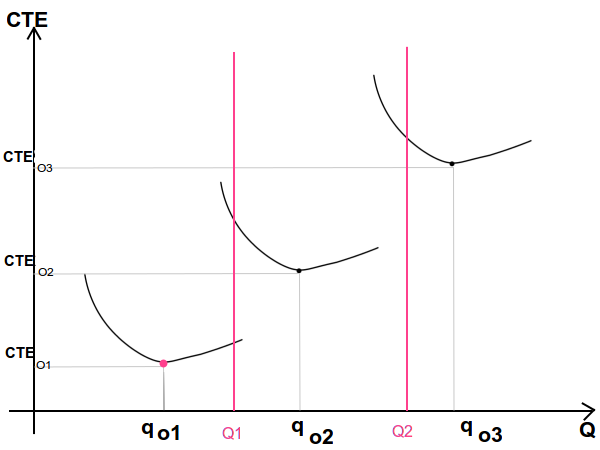
\includegraphics[scale=0.5,keepaspectratio=true]{img/8/8_QvsCTE_1.png} 
 \item sino, si $q_{o2} < Q_2 \Rightarrow CTE_o = min( CTE_{o2}, CTE(Q_1, k_1)) $ \\
      Se entiende por $CTE(Q_i, k_i)$ el costo total esperado \eqref{8_CTE} evaluado en $Q_i$ y $k_i$ \\
      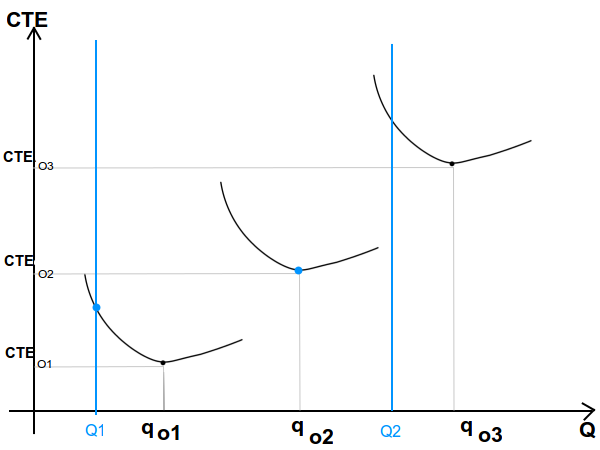
\includegraphics[scale=0.5,keepaspectratio=true]{img/8/8_QvsCTE_2.png} 
 \item sino, $q_{o3} > Q_2 \Rightarrow CTE_o = min( CTE_{o3}, CTE(Q_2, k_2), CTE(Q_1, k_1) )$ \\
      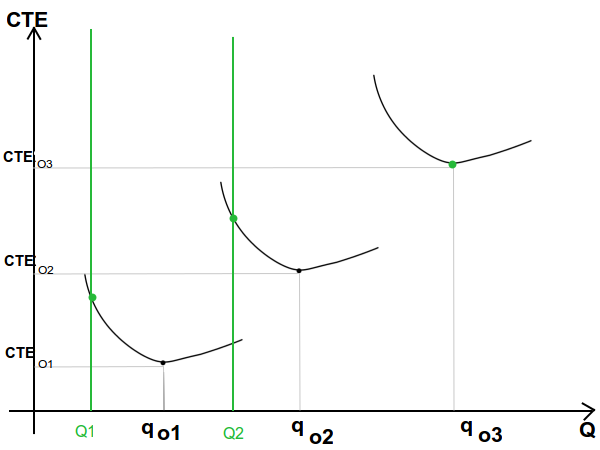
\includegraphics[scale=0.5,keepaspectratio=true]{img/8/8_QvsCTE_3.png} 
\end{enumerate}

Dado que cada curva es válida únicamente en un intervalo determinado por k, para cada caso el CTE en función de q está dado por la curva naranja.\\
\begin{enumerate}
  \item 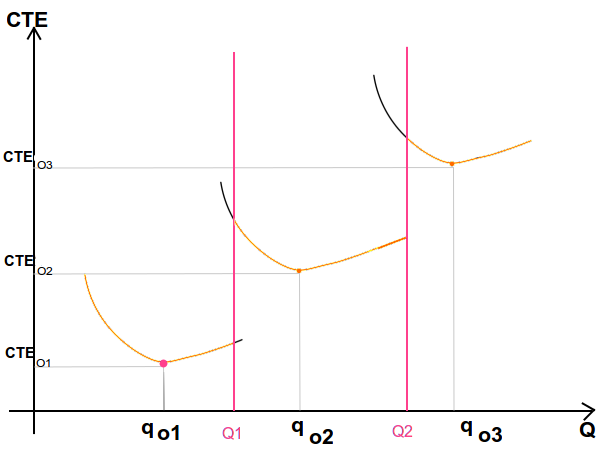
\includegraphics[scale=0.5,keepaspectratio=true]{img/8/8_QvsCTE_1b.png} 
  \item 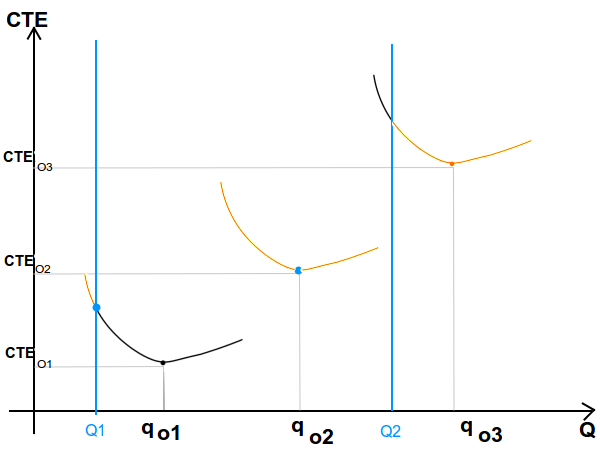
\includegraphics[scale=0.5,keepaspectratio=true]{img/8/8_QvsCTE_2b.png} 
  \item 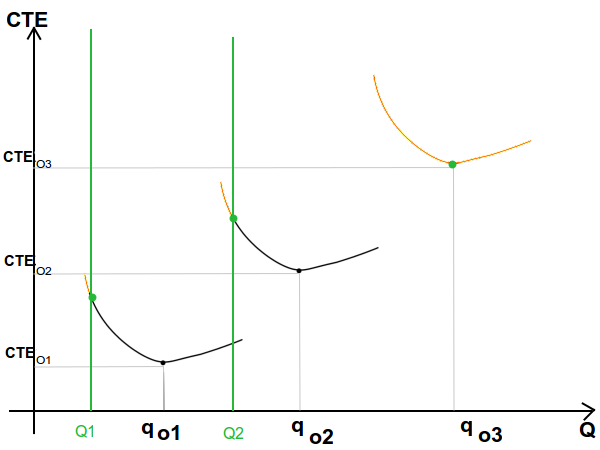
\includegraphics[scale=0.5,keepaspectratio=true]{img/8/8_QvsCTE_3b.png} 
\end{enumerate}

\end{document}
